\documentclass[11pt]{article}

\usepackage[margin=1in]{geometry}
\usepackage[T1]{fontenc}
\usepackage[utf8]{inputenc}
\usepackage{lmodern}
\usepackage{amsmath,amssymb,mathtools}
\usepackage{booktabs}
\usepackage{graphicx}
\usepackage{array}
\usepackage{enumitem}
\usepackage[hidelinks]{hyperref}
\usepackage{microtype}

\title{SimpleSFT Project Report}
\author{Dylan Tan \and Oliver Proudfoot}
\date{\today}

\newcommand{\bytes}[1]{\operatorname{bytes}\!\left(#1\right)}
\newcommand{\ind}[1]{\mathbb{1}\!\left[#1\right]}

\begin{document}
\maketitle

\begin{abstract}
SimpleSFT estimates whether supervised fine-tuning jobs for popular research
LLMs, including Qwen-family models, will fit on available GPU resources before
launch. The project combines a typed analytical memory model, CUDA-based
measurement tools, saved benchmark comparisons, and configuration search.
A user-friendly web UI recommends training strategies based on the estimator's output and exports
a TRL-compatible YAML strategy for the selected configuration. The current
estimator shows a global mean absolute error of 1.332 GiB and a median relative
error of 6.1\% on a saved measurement corpus, which is strong for pre-launch
screening when users keep 10\% headroom.
\end{abstract}

\begin{center}
\small
\textbf{Project repository:} \url{https://github.com/olliepro/SimpleSFT}
\end{center}

\section{Project Goal}
SimpleSFT estimates the memory requirements for supervised fine-tuning (SFT) jobs
on popular large language models (LLMs) used in academic research. These models
include open-weight Qwen-family models, OLMo, LLaMA, and Mistral, which are common in current research
workflows and span sizes where a small change in distributed strategy can
determine whether a job runs at all.

\begin{quote}
Given a model, context length, resource pool, and training strategy, estimate
the expected per-rank peak memory and identify the training phase that produces
that peak.
\end{quote}

Today, users face slow trial-and-error development workflows to find parallel
strategies that meet their specific needs: short debug allocations on OSC
allow only one GPU, while larger allocations can require long queues or long reservations.
SimpleSFT helps users choose a plausible strategy before occupying GPUs for extended setup runs.

The state of OSC queues is often unpredictable and frustrating. This has led to a culture of
overprovisioning, where users request more resources than they expect to need just to be
sure they will have time to debug their jobs. This is inefficient for everyone: users wait
longer in queues, and the cluster is less available for other work. SimpleSFT provides a
more informed way to request resources, which can reduce wait times and improve overall
cluster efficiency.

This framing matters on shared academic clusters. An NLP researcher seeking to do SFT often begins
with a concrete scientific question, a model family, and some training data. The act of
engineering a system to run SFT efficiently is incidental to the true research question.
SimpleSFT lightens that work by providing a framework for getting to model training with less trial and error.

\section{System Overview}
The project has four main pieces:
\begin{itemize}[leftmargin=1.4em]
\item \textbf{Model inspection:} Hugging Face models are summarized as a
\texttt{ModelSpec}: layer count, hidden and intermediate sizes, vocabulary,
attention layout, parameter shapes, trainable linear layers, tensor-layout
roles, and optional architecture metadata.
\item \textbf{Analytical estimation:} an \texttt{EstimatorConfig} describes the
training strategy. The estimator builds resident state, retained activations,
workspace windows, and phase peaks, then returns a \texttt{MemoryResult}.
\item \textbf{Measurement and saved comparisons:} CUDA microsteps provide
ground-truth memory measurements for selected configurations. The saved
measurements let later estimator changes be checked against the same cases.
\item \textbf{Workflow tools:} CLI and local web paths expose estimate, search,
measure, compare, benchmark, report, YAML export, and SFT launch commands.
\end{itemize}

\section{Estimator Model}
SimpleSFT treats a training step as three candidate peaks:
\[
M_{\mathrm{peak}} =
\max(M_{\mathrm{forward}}, M_{\mathrm{backward}}, M_{\mathrm{optimizer}}).
\]
Forward starts from parameters and runtime support. Backward adds gradients and
backward-live activation state. The optimizer step adds update scratch,
communication buckets, and phase carryover. This breakdown gives a useful
structure for model design and calibration because each estimator change can be
attached to a specific phase and memory family.

\subsection{Inputs}
The estimator combines a \texttt{ModelSpec} and an \texttt{EstimatorConfig}.
The model spec supplies architecture and tensor metadata: parameter shapes,
linear-layer roles, attention widths, vocabulary size, layer count, and
tensor-parallel layout annotations. The config supplies the training strategy:
tuning mode, optimizer, dtypes, sequence length, GPU budget, attention backend,
checkpointing, LoRA settings, distributed mode, tensor and sequence parallel
choices, runtime-support assumptions, and DDP/ZeRO bucket sizes.

The inspected model metadata is highly detailed. For a
Qwen-style model, the estimator needs the number of transformer blocks, the
hidden width, the MLP expansion width, the number of attention heads, the number
of key/value heads, the vocabulary projection shape, and the local role of each
large matrix under tensor parallelism. The same total parameter count can lead
to different memory behavior when the attention projection layout, MLP layout,
or vocabulary tensor is sharded differently.

\begin{center}
\small
\begin{tabular}{@{}p{0.28\linewidth}p{0.62\linewidth}@{}}
\toprule
Estimator input & Why it affects peak memory \\
\midrule
Parameter shapes & Drive parameter bytes, gradient bytes, optimizer state, and
tensor-parallel local ownership. \\
Linear-layer list & Identifies LoRA target modules and adapter parameter
counts. \\
Attention layout & Determines query and key/value widths, attention workspace,
and long-context retained state. \\
Distributed strategy & Changes rank ownership of gradients, optimizer state,
parameters, buckets, and gather windows. \\
Checkpointing flag & Changes retained activation state and adds backward
recompute workspace. \\
\bottomrule
\end{tabular}
\normalsize
\end{center}

\subsection{Resident State}
Resident state is the memory floor on one rank:
\[
R_{\mathrm{base}} =
M_{\mathrm{params}} + M_{\mathrm{opt}} + M_{\mathrm{master}}
+ M_{\mathrm{runtime}} + M_{\mathrm{persist}},
\qquad
R_{\mathrm{grad}} = R_{\mathrm{base}} + M_{\mathrm{grads}}.
\]
Parameters are counted from explicit parameter shapes when available, with
tensor-parallel sharding applied to row, column, and vocabulary-parallel
tensors. ZeRO-3 shards trainable parameters across data-parallel ranks. LoRA
keeps the dense base weights resident and makes the adapter tensors trainable,
so gradients and optimizer state scale with adapter size.

Optimizer memory is optimizer-specific. Adam and AdamW keep two state tensors,
RMSProp and Adagrad keep one, SGD keeps none, and Adafactor uses factored state
for matrix-like tensors. ZeRO-2 and ZeRO-3 shard optimizer state and gradients
for tested optimizer paths. Runtime support is represented with named CUDA,
allocator, NCCL, DeepSpeed, and backend-buffer terms.

The local tensor count is computed before bytes are assigned. Tensor-parallel
metadata determines whether a parameter is replicated or divided across the
tensor-parallel group. ZeRO then applies data-parallel sharding to the training
state owned by its stage. This order preserves the difference between a matrix
partitioned by tensor parallelism and a state object partitioned by ZeRO.

\begin{center}
\small
\begin{tabular}{@{}lll@{}}
\toprule
Object & Full fine-tuning & LoRA fine-tuning \\
\midrule
Base weights & resident & resident \\
Trainable weights & dense model tensors & adapter tensors \\
Gradients & dense trainable tensors & adapter gradients \\
Optimizer state & dense trainable tensors & adapter optimizer state \\
\bottomrule
\end{tabular}
\normalsize
\end{center}

This distinction is central for LLMs, because a full fine-tune must carry
optimizer and gradient state for the dense model. A LoRA run still stores the
base weights during forward and backward passes, while trainable-state memory demand is determined by
the targeted projection layers and the selected adapter rank.

For one dense matrix $W \in \mathbb{R}^{d_{\mathrm{out}}\times d_{\mathrm{in}}}$,
full fine-tuning makes all $d_{\mathrm{out}}d_{\mathrm{in}}$ elements trainable.
LoRA inserts
\[
\Delta W = \frac{\alpha}{r}BA,\qquad
A \in \mathbb{R}^{r\times d_{\mathrm{in}}},\quad
B \in \mathbb{R}^{d_{\mathrm{out}}\times r},
\]
so the trainable count for that target becomes
$r(d_{\mathrm{in}} + d_{\mathrm{out}})$. The dense base matrix remains part of
resident parameter memory, while gradient and optimizer memory follow the
adapter tensors. This gives the estimator a direct way to reason about rank,
target module selection, and optimizer state without introducing a separate
LoRA-only formula for the rest of the model.

Optimizer state is handled at parameter-tensor granularity. Adam-style
optimizers attach two state tensors to each trainable tensor. Adafactor uses
row and column factors for matrix-like tensors, which is materially smaller for
large projection matrices. This tensor-level treatment matters for mixed
training modes: a run can have dense frozen base parameters, trainable adapter
matrices, and optimizer state only for those adapters.

\subsection{Retained Activations and Attention}
Retained activation memory is a sum of terms:
\[
M_{\mathrm{act}} =
M_{\mathrm{visible}} + M_{\mathrm{saved\ inputs}} + M_{\mathrm{mlp}}
+ M_{\mathrm{attn}} + M_{\mathrm{lora}} + M_{\mathrm{ckpt}}
+ M_{\mathrm{loss}} + M_{\mathrm{widened}}.
\]
Full fine-tuning grows with layer count, local token count, hidden width, MLP
width, and attention-path width. LoRA reduces trainable activation pressure by
moving gradients onto targeted adapter paths and low-rank intermediates.
Gradient checkpointing stores fewer layer internals and shifts work into
backward recomputation.

Attention backend matters most at long context length. Standard attention
requires attention-score states that scale quadratically with sequence length.
FlashAttention removes the need to store quadratic-length attention scores by
using tiled computation and recomputation, with a smaller additional workspace
term \cite{dao2022flashattention}. SimpleSFT therefore models FlashAttention
primarily through retained attention-path context and workspace terms.

Gradient checkpointing is modeled as a change to the activation life cycle.
Layer internals that would be retained until backward are reduced, while a
separate recompute window is added during backward. The estimator represents
this through checkpoint-boundary bytes, saved linear-input bytes, residual and
normalization context, and recompute workspace. This keeps the memory tradeoff
visible: checkpointing lowers retained forward state and raises backward
compute plus transient workspace.

\subsection{Workspace and Phase Assembly}
Workspace is modeled as a live window. The main terms are attention workspace,
backward kernel workspace, recompute workspace, loss workspace, tensor/sequence
parallel communication windows, optimizer update scratch, and distributed
bucket objects.

DDP contributes a reducer bucket and a communication-overlap window. ZeRO
contributes all-gather, reduce, and prefetch buckets. Bucket capacities are
derived from configured element counts and clipped by the local payload that
can fill them. ZeRO optimizer pressure is the maximum of fetch, update, and
communication subphases.

The bucket model uses configured capacities and local payload caps. A reducer
or all-gather bucket can reserve a large object, yet the active payload remains
bounded by the data held on that rank. This makes the estimate responsive to
both runtime settings and model size. ZeRO-2 keeps parameters resident while
sharding optimizer state and gradients. ZeRO-3 also shards trainable
parameters, adding parameter gather windows around computation.

The final phase equations are:
\[
\begin{aligned}
M_{\mathrm{forward}} &= R_{\mathrm{base}} + A_{\mathrm{fwd}} + W_{\mathrm{fwd}}, \\
M_{\mathrm{backward}} &= R_{\mathrm{grad}} + A_{\mathrm{bwd}} + W_{\mathrm{bwd}}, \\
M_{\mathrm{optimizer}} &=
R_{\mathrm{grad}} + E_{\mathrm{bwd}} + W_{\mathrm{opt}} + C_{\mathrm{opt}}.
\end{aligned}
\]
Here $E_{\mathrm{bwd}}$ is backward-end state such as gradients and live
distributed buckets, and $C_{\mathrm{opt}}$ represents carryover that remains
live at optimizer-step entry.

The phase assembly makes the peak source explicit. A forward peak usually
signals parameter plus retained activation pressure. A backward peak usually
signals the combination of gradients, retained or recomputed activations, and
communication workspace. An optimizer-step peak usually signals optimizer
state, update scratch, and ZeRO communication windows. Reporting this phase is
important because two configurations can have similar total peaks while needing
different fixes. For example, checkpointing helps a forward-activation peak,
while ZeRO stage changes help persistent optimizer or gradient pressure.

\begin{center}
\small
\begin{tabular}{@{}p{0.22\linewidth}p{0.68\linewidth}@{}}
\toprule
Peak phase & Dominant terms SimpleSFT reports \\
\midrule
Forward & Base resident state, retained activations, attention workspace,
loss-related state. \\
Backward & Resident state with gradients, backward activation state,
checkpoint recompute workspace, DDP or ZeRO communication windows. \\
Optimizer step & Gradients, optimizer state, update scratch, ZeRO fetch and
communication windows, carried state from backward. \\
\bottomrule
\end{tabular}
\normalsize
\end{center}

\section{Strategy Selection and User Workflow}
The estimator can answer one fixed-configuration question or search over a
small set of feasible strategies. A candidate is an \texttt{EstimatorConfig}
paired with a resolved \texttt{ModelSpec}. The CLI search path evaluates the
requested resource and distributed-mode options, separates feasible and
infeasible cases, and ranks candidates by feasibility, distributed-mode
simplicity, and memory headroom.

The simplicity order is:
\[
\texttt{tp\_only}
\prec
\texttt{ddp}
\prec
\texttt{zero2}
\prec
\texttt{zero3}.
\]
This favors a smaller distributed stack when the memory estimate permits it.
The UI uses a richer candidate set over distributed mode,
checkpointing, tensor-parallel degree, and sequence-parallel settings. DDP and
ZeRO require enough GPUs for data parallelism after tensor parallelism is
assigned, while sequence parallelism requires tensor parallelism.

Candidate generation follows the same constraints a user would apply by hand.
The resource pool determines the available GPU count and memory budget. Tensor
parallelism consumes GPUs inside each model replica. Data parallelism then uses
the remaining replica count. ZeRO stages are considered only when a data
parallel group exists. Sequence parallelism is paired with tensor parallelism,
since it partitions sequence-local activation state across the tensor-parallel
group.

\begin{center}
\small
\begin{tabular}{@{}p{0.25\linewidth}p{0.65\linewidth}@{}}
\toprule
Strategy family & Search treatment \\
\midrule
Single GPU & Used when only one GPU is specified. \\
Tensor parallel & Shards eligible matrices and associated tensor-local state
across the tensor-parallel group. \\
DDP & Replicates model state and changes communication workspace through
reducer buckets. \\
ZeRO-2 & Shards gradients and optimizer state across data-parallel ranks. \\
ZeRO-3 & Shards trainable parameters as well, adding gather and prefetch
windows around computation. \\
LoRA & Changes trainable tensors and optimizer state through adapter rank and
target modules. \\
\bottomrule
\end{tabular}
\normalsize
\end{center}

Among feasible results, the reported headroom gives the user a practical margin against
allocator variation, dataloader details, and small differences between the
synthetic estimate and the real training script. The search output therefore
contains both the selected candidate and the alternatives, allowing a user to
choose a slower option with more margin when the cluster allocation is scarce.

\subsection{Slowdown Model}
Slowdown estimation is separate from memory estimation. The web recommendation
path uses a small heuristic prior:
\[
R_{\mathrm{slow}} =
\left(1 + s_{\mathrm{dist}}\right)
\left(1 + s_{\mathrm{ckpt}}\right)
\left(1 + s_{\mathrm{tp}}\right)
\left(1 + s_{\mathrm{sp}}\right) - 1.
\]
The distributed-mode priors are $0\%$ for single-GPU and pure tensor
parallelism, $3\%$ for DDP, $8\%$ for ZeRO-2, and $18\%$ for ZeRO-3.
Checkpointing contributes $30\%$ because recomputation increases backward
work. Tensor parallelism contributes $0.08\log_2(T_{\mathrm{P}})$, and
sequence parallelism contributes $4\%$ when enabled.

The slowdown score is simple because estimating training time is a hard problem
outside the scope of this project. It expresses the expected slowdown
relative to the least-sharded feasible candidate.
For example, checkpointing receives a large penalty because it trades memory for
extra backward compute. ZeRO-3 receives a larger distributed penalty than
ZeRO-2 because parameter gathering introduces additional synchronization and
workspace.

\subsection{Training Export}
Search results can be exported into a TRL-compatible YAML strategy. The export
contains the model reference, tuning mode, optimizer and precision choices,
sequence length, checkpointing, attention backend, distributed strategy, and
LoRA fields when applicable. The training runner consumes the first exported
candidate by default. In the intended workflow, the user searches over model,
context length, resource pool, and distributed strategy, exports the best
candidate, and launches training from that file:

\begin{verbatim}
simplesft search <HF Model> ... --export-file ./trl_strategy.yaml
simplesft train --config ./trl_strategy.yaml --dataset <HF Dataset>
\end{verbatim}

The command-line interface and web server return the same core objects: peak
memory, feasibility, phase records, component breakdowns, assumptions, and
diagnostic metadata.

\section{Measurement and Evaluation Method}
As a ground-truth target for estimator development, we measured the memory usage
of various parallel training strategies. SimpleSFT runs
real CUDA microsteps and records memory use around the training phases that the
analytical model predicts. Measurements are collected once, saved with their configurations, and
used during analytical model calibration.

DDP runs use \texttt{torchrun}. Each rank measures its own local microstep,
serializes a \texttt{MemoryResult}, and rank zero stores a conservative
max-across-ranks aggregate. ZeRO-2 and ZeRO-3 use a DeepSpeed launcher with the
same stage, bucket, prefetch, overlap, reduce-scatter, all-gather, and precision
settings used by the estimator. Single-rank ZeRO measurement is rejected
because sharding requires more than one rank.

The measured breakdown records live parameter bytes, gradient bytes,
optimizer-state bytes, retained activation bytes, runtime reserve, and
transient remainder. Synthetic text batches keep the sequence length and label
shape controlled across runs.

\section{Quantitative Accuracy}
The current saved measurement corpus covers 324 rows of various run configurations. The global error is small enough for practical feasibility screening while leaving room for improvement in runtime lifetime modeling.

\begin{align*}
\text{Global MAE} &= 1.332\ \mathrm{GiB} \\
\text{Mean Absolute Relative Error} &= 9.1\% \\
\text{Median Absolute Relative Error} &= 6.1\% \\
\text{Retained-Forward Proxy MAE} &= 1.101\ \mathrm{GiB}
\end{align*}

The most useful interpretation of these numbers is operational. An estimate
with several GiB of headroom is usually enough to decide whether a launch
configuration is plausible. Tight fits still need measured confirmation,
especially when a strategy relies on ZeRO, checkpointing, or long-context.

\section{Limitations and Future Work}
Several parts of the estimator still depend on calibrated runtime assumptions.
Runtime support and optimizer-step carryover are fudge terms that account for memory overhead outside the analytical model's current coverage.
Additionally, the slowdown score used for recommendations should become a measured timing model.

The next technical step is to connect timing and memory in the same artifact.
The memory estimator already ranks feasibility well enough for pre-launch
screening. A measured timing model would make slowdown estimates less
heuristic, especially for ZeRO-3, checkpointing, and tensor-parallel jobs where
communication and recomputation dominate user-visible cost.

\section{Related Work}
SimpleSFT follows prior work on memory-aware fine-tuning and distributed
training while targeting a narrower workflow: fast SFT strategy selection on
research LLMs before launch. LLMem estimates memory for distributed
fine-tuning and recommends methods for multi-GPU LLM training
\cite{kim2024llmem}, but it lacks modern attention backends and support for LoRA. Empirical work on distributed Transformer training
studies how model architecture and distributed strategy interact with memory
and performance \cite{lu2024distributed}. Broader resource-management work
compares analytical, CPU-side, and learning-based estimators for GPU memory and
utilization \cite{yousefzadeh2026gpu}. SimpleSFT uses the same general
motivation, then adds project-specific measurement artifacts and SFT-oriented
strategy export.

\begin{center}
\small
\begin{tabular}{@{}>{\raggedright\arraybackslash}p{0.31\linewidth}p{0.59\linewidth}@{}}
\toprule
Work & Relationship to SimpleSFT \\
\midrule
LLMem \cite{kim2024llmem} & Analytical GPU-memory estimation for LLM
fine-tuning and method recommendation across distributed training settings. It was calibrated using older models and different data regimes. \\
Transformer training study \cite{lu2024distributed} & Empirical view of
memory and performance behavior under distributed training choices. \\
Training-aware resource management \cite{yousefzadeh2026gpu} & Broader
resource-management framing for memory and utilization prediction. \\
\bottomrule
\end{tabular}
\normalsize
\end{center}

This work builds directly on prior work in training optimization. LoRA
reduces trainable state by injecting low-rank adapter matrices into frozen base
models \cite{hu2021lora}. ZeRO shards redundant training state across data
parallel ranks \cite{rajbhandari2020zero}. FlashAttention changes the memory
shape of attention through IO-aware tiling that avoids the full quadratic score
matrix \cite{dao2022flashattention}. These methods are common in current LLM
fine-tuning practice, including Qwen-family research workflows \cite{qwen25}.

\section{Conclusion}
SimpleSFT gives researchers a practical way to plan SFT jobs before reserving
scarce GPU time. The estimator connects inspected model structure with
distributed training choices, LoRA, checkpointing, FlashAttention, optimizer
state, and CUDA runtime support. The result is a phase-level estimate that can
guide resource selection and clarify the expected source of memory pressure.

The current saved measurement corpus shows a global mean absolute error of
1.332 GiB and a median relative error of 6.1 percent. Those numbers are strong
for pre-launch screening, especially when users keep several GiB of memory
headroom.

\bibliographystyle{plain}
\bibliography{references}

\clearpage
\appendix
\section{Web Interface Screenshot}
\begin{figure}[h]
\centering
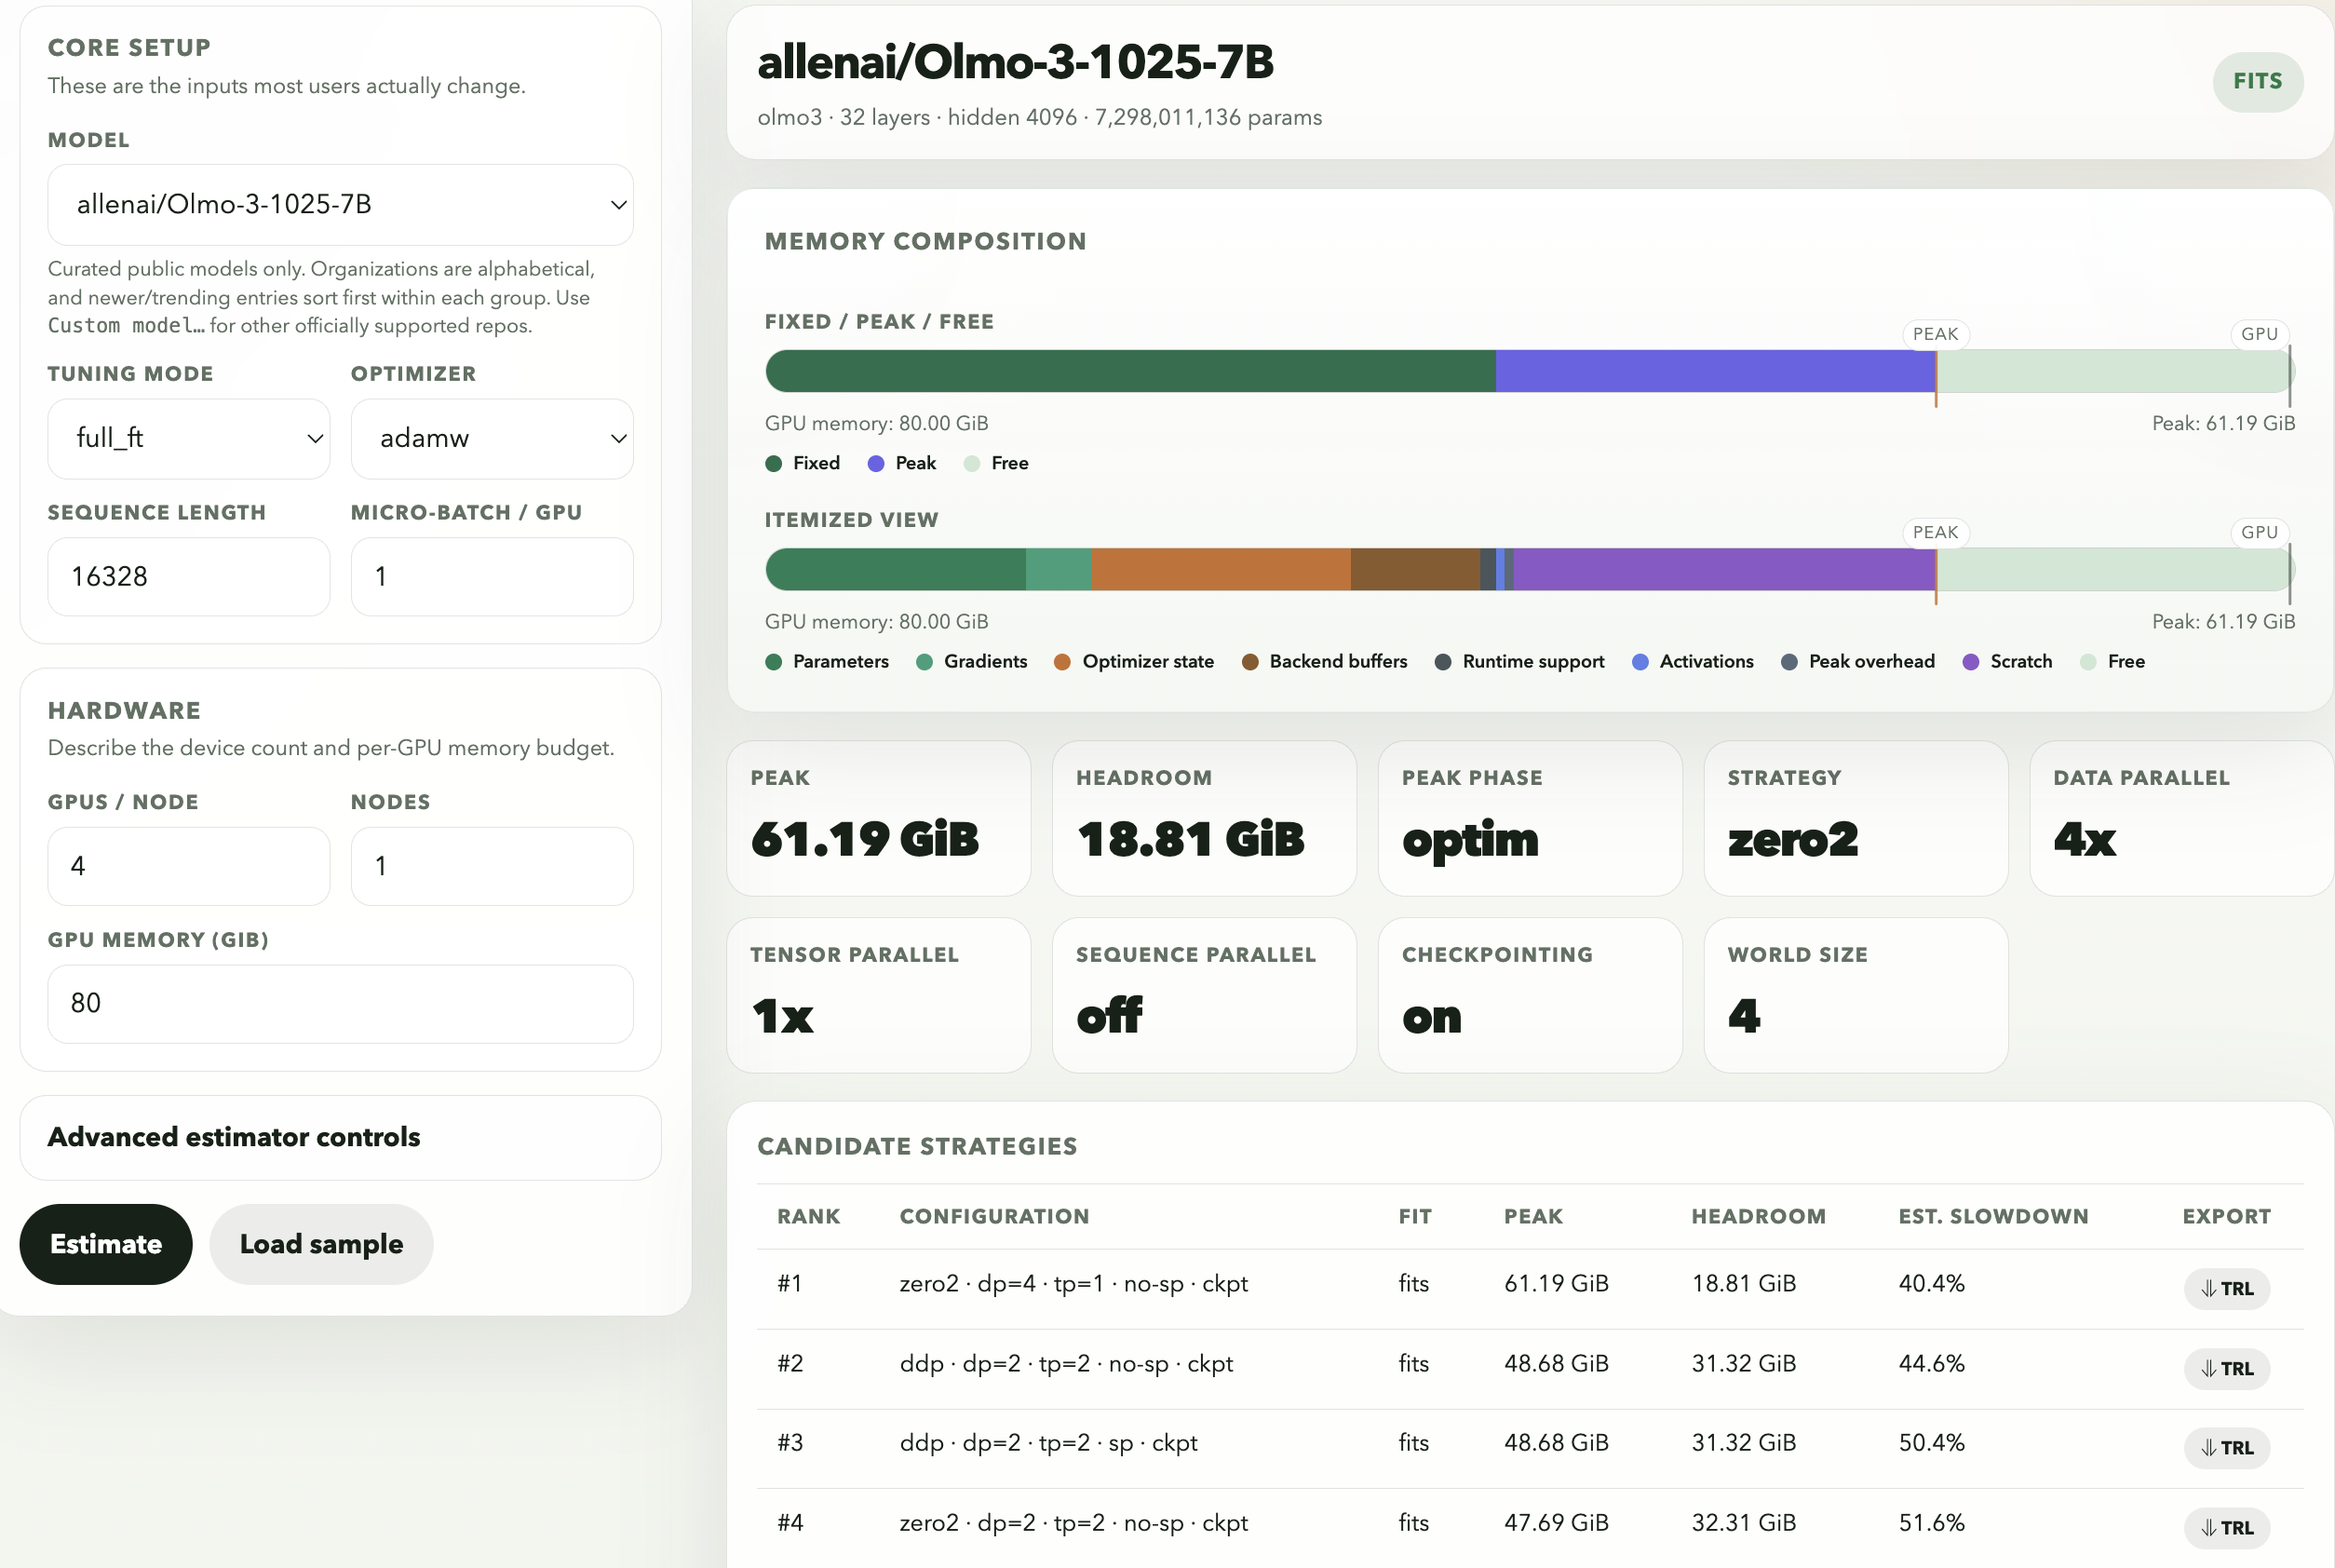
\includegraphics[width=\textwidth,height=0.82\textheight,keepaspectratio]{sections/image.png}
\caption{SimpleSFT web interface showing an example estimate and ranked candidate strategies.}
\label{fig:web-interface-screenshot}
\end{figure}

\end{document}
